\documentclass{article}

\usepackage{amssymb, amsmath, amsthm, graphicx, tikz, tikz-3dplot}
\usepackage[colorlinks = false]{hyperref}
\hypersetup{pdfborder = {0 0 0}}

\usepackage[procnames]{listings}
\lstset{basicstyle=\ttfamily, language=TeX, frame=single}

\title{Graphics}
\date{}

\begin{document}

\maketitle

There is no substitute for high quality graphics.  If a technical
topic is visual in nature, much time and attention should be paid
to creating powerful images.  A good image communicates
information more easily than the printed word.

\section{Including outside images}

Images can be included using the \verb~graphicx~ package (loaded
in the preamble).  Include an image using
\verb~\includegraphics[options]{file}~ where \verb~file~ can be a
file in \verb~.pdf~, \verb~.jpg~, or \verb~.png~ format.
Available \verb~options~ are
\begin{center}
  \begin{tabular}{r l}
    \verb~width = X~  & to specify a width \verb~X~     \\
    \verb~height = X~ & to specify height \verb~X~      \\
    \verb~scale = X~  & to scale by multiplier \verb~X~ \\
    \verb~angle = X~  & to rotate counter-clockwise by \verb~X~ degrees
  \end{tabular}
\end{center}
For example, the image
\begin{center}
  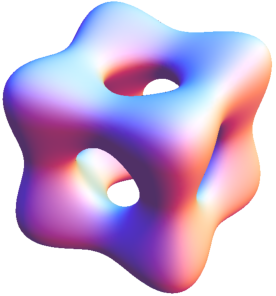
\includegraphics[scale = 1.25]{351Week6HolyCube}
\end{center}
was created in Mathematica by plotting the set of $x,y,z$
coordinates in $\mathbb{R}^3$ which satisfy
\(x^4+y^4+z^4 + 3/8 = x^2+y^2+z^2 \).  It was saved as
\verb~351Week6HolyCube.pdf~ and then shown here using
\verb~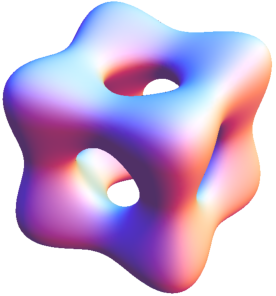
\includegraphics[scale = 1.25]{351Week6HolyCube}~.

\section{TikZ}

TikZ can produce graphics of excellent quality.  It can do lots of
things, but there is an initial time investment necessary to
understand TikZ code.

This document does not attempt to give a good description---or even
a coherent introduction---to creating graphics with TikZ.  For those
purposes, refer to the short ``Minimal introduction to TikZ'' and
the long ``PGF manual'' found
at \url{https://www.ctan.org/pkg/pgf}.  Instead, this document
will display some of TikZ's abilities with a few well chosen
examples.  Many more interesting examples are available
at \url{http://www.texample.net/tikz/examples/}.

To use TikZ, load the package \verb~tikz~ in the preamble and then
place TikZ code in the \verb~tikzpicture~ environment.

Think about TikZ code as doing two things:
\begin{enumerate}
\item identifying some $(x,y)$ coordinates, and
\item describing how to connect those points.
\end{enumerate}

The \verb~\draw~ command draws lines connecting a list of $(x,y)$
coordinates separated by the \verb~--~ delimiter.  The
\verb~\draw~ command and all other TikZ commands must end with a
semicolon.  Optional commands to \verb~\draw~ are called using
brackets.  One of the many such options is \verb~rounded corners~,
which gives rounded corners.

\begin{lstlisting}
  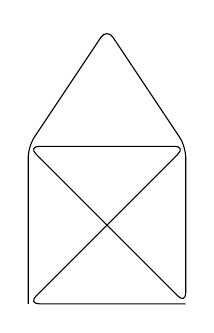
\begin{tikzpicture}
    \draw [rounded corners] (0,0) -- (0,2) -- (1,3.5) --
    (2,2) -- (2,0) -- (0,2) -- (2,2) -- (0,0) -- (2,0);
  \end{tikzpicture}
\end{lstlisting}

\begin{center}
  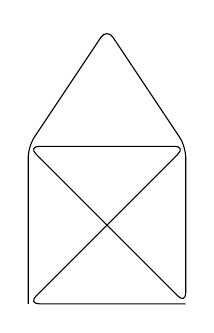
\begin{tikzpicture}
    \draw [rounded corners] (0,0) -- (0,2) -- (1,3.5) -- (2,2) -- (2,0) -- (0,2) --
    (2,2) -- (0,0) -- (2,0);
  \end{tikzpicture}
\end{center}

Simple functions like polynomials and trigonometric functions can be plotted
using ``plot'' within \verb~\draw~ command; below is the graph of
$-x^2 + x + 1$ on $[0,2]$:

\begin{lstlisting}
  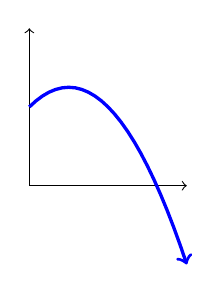
\begin{tikzpicture}
    \draw [->] (0,0) -- (2,0);
    \draw [->] (0,0) -- (0,2);
    \draw [blue, very thick, domain=0:2, ->]
    plot (\x, {-1*pow(\x, 2) + \x + 1});
  \end{tikzpicture}
\end{lstlisting}

\begin{center}
  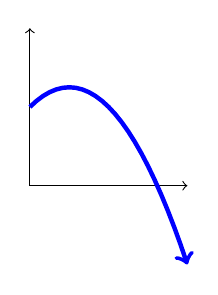
\begin{tikzpicture}
    \draw [->] (0,0) -- (2,0);
    \draw [->] (0,0) -- (0,2);
    \draw [blue, ultra thick, domain=0:2, ->] plot (\x, {-1*pow(\x, 2) + \x + 1});
  \end{tikzpicture}
\end{center}

Parametric equations can also be graphed; for instance, to graph the parametric
equations $(\cos ( 4 t) + \cos t, \sin ( 4 t) + \sin t)$ for $t \in [0,2 \pi]$, do
this:

\begin{lstlisting}
  \begin{tikzpicture}[scale = .9]
    \draw [domain=0:2*pi,
    samples = 150,

    fill = orange]
    plot ({cos(4*\x r) + cos(\x r)},
    {sin(4*\x r) + sin(\x r)});
  \end{tikzpicture}
\end{lstlisting}

\begin{center}
  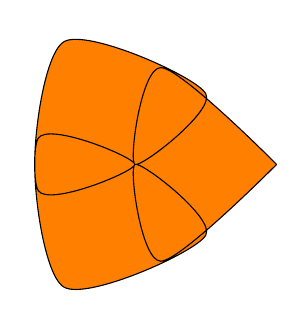
\begin{tikzpicture}[scale = .9]
    \draw [domain=0:2*pi,
    samples = 13,
    smooth,
    fill = orange]
    plot ({cos(4*\x r) + cos(\x r)},
    {sin(4*\x r) + sin(\x r)});
  \end{tikzpicture}
\end{center}
The \verb~r~ in \verb~cos(4*\x r)~ indicates that \verb~\x~ is in radians, not
degrees.  For complicated curves without a simple formula it is best to use
outside software to generate a lots of $(x,y)$ coordinates which can then be
called with \verb~\draw~.

The $(x,y)$ coordinates can be given names and labels using the \verb~\node~
command, in this way:

\begin{lstlisting}
  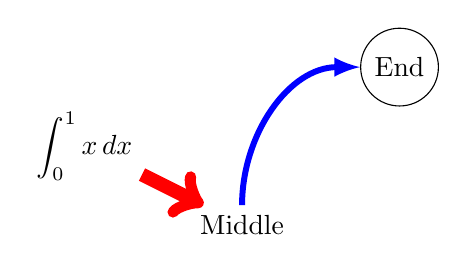
\begin{tikzpicture}
    \node (A) at (0,0) {$\displaystyle \int_0^1 x \, dx$};
    \node (B) at (2,-1) {Middle};
    \node [draw, circle] (C) at (4,1) {End};
    \draw [line width=.5em, ->, red] (A) -- (B);
    \draw [line width=.5ex, -latex, blue] (B)
    to [out=90, in=180] (C);
  \end{tikzpicture}
\end{lstlisting}

\begin{center}
  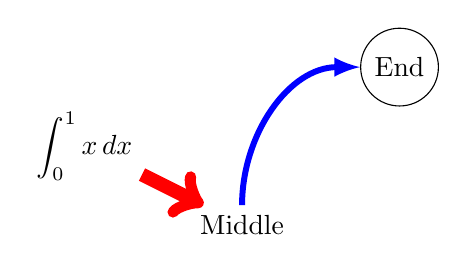
\begin{tikzpicture}
    \node (A) at (0,0) {$\displaystyle \int_0^1 x \, dx$};
    \node (B) at (2,-1) {Middle};
    \node [draw, circle] (C) at (4,1) {End};
    \draw [line width=.5em, ->, red] (A) -- (B);
    \draw [line width=.5ex, -latex, blue] (B)
    to [out=90, in=180] (C);
  \end{tikzpicture}
\end{center}

This last example used a slightly different syntax in the
\verb~\draw~ command; instead of using a \verb~--~ delimiter, the
command \verb~to~ was used, which contains the option of
specifying the outgoing and incoming angles in degrees.

The remainder of this document displays good examples of TikZ
figures.  The generating code can be found in the \LaTeX{}
\verb~.tex~ file.

\begin{center}
  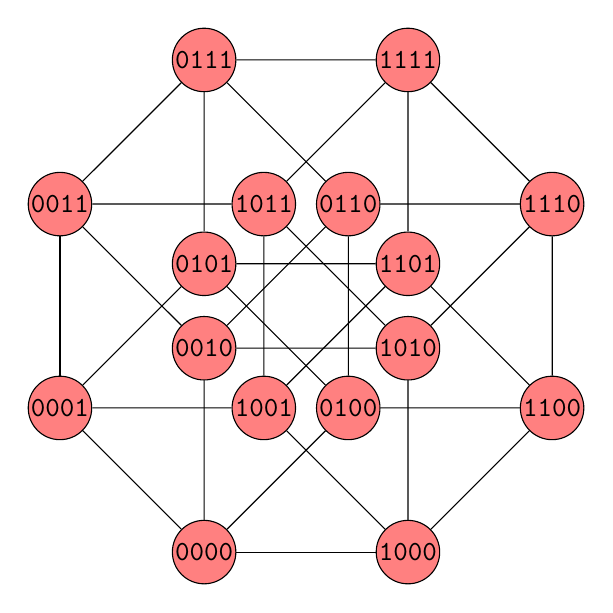
\begin{tikzpicture}[scale=1.25]
    \tikzstyle{every node} = [draw, circle, fill = red!50, inner sep = .1ex];
    \node (v0) at (1.4645,0) {\texttt{0000}};
    \node (v1) at (0.0,1.4645) {\texttt{0001}};
    \node (v2) at (1.4645,2.0711) {\texttt{0010}};
    \node (v3) at (0.0,3.5355) {\texttt{0011}};
    \node (v4) at (2.9289,1.4645) {\texttt{0100}};
    \node (v5) at (1.4645,2.9289) {\texttt{0101}};
    \node (v6) at (2.9289,3.5355) {\texttt{0110}};
    \node (v7) at (1.4645,5.0) {\texttt{0111}};
    \node (v8) at (3.5355,0.0) {\texttt{1000}};
    \node (v9) at (2.0711,1.4645) {\texttt{1001}};
    \node (v10) at (3.5355,2.0711) {\texttt{1010}};
    \node (v11) at (2.0711,3.5355) {\texttt{1011}};
    \node (v12) at (5.0,1.4645) {\texttt{1100}};
    \node (v13) at (3.5355,2.9289) {\texttt{1101}};
    \node (v14) at (5.0,3.5355) {\texttt{1110}};
    \node (v15) at (3.5355,5.0) {\texttt{1111}};
    \draw (v0) -- (v1);
    \draw (v0) -- (v2);
    \draw (v0) -- (v4);
    \draw (v0) -- (v8);
    \draw (v1) -- (v3);
    \draw (v1) -- (v5);
    \draw (v1) -- (v9);
    \draw (v2) -- (v3);
    \draw (v2) -- (v6);
    \draw (v2) -- (v10);
    \draw (v3) -- (v7);
    \draw (v3) -- (v11);
    \draw (v4) -- (v5);
    \draw (v4) -- (v6);
    \draw (v4) -- (v12);
    \draw (v5) -- (v7);
    \draw (v5) -- (v13);
    \draw (v6) -- (v7);
    \draw (v6) -- (v14);
    \draw (v7) -- (v15);
    \draw (v8) -- (v9);
    \draw (v8) -- (v10);
    \draw (v8) -- (v12);
    \draw (v9) -- (v11);
    \draw (v9) -- (v13);
    \draw (v10) -- (v11);
    \draw (v10) -- (v14);
    \draw (v11) -- (v15);
    \draw (v12) -- (v13);
    \draw (v12) -- (v14);
    \draw (v13) -- (v15);
    \draw (v14) -- (v15);
  \end{tikzpicture}
\end{center}

\begin{center}
  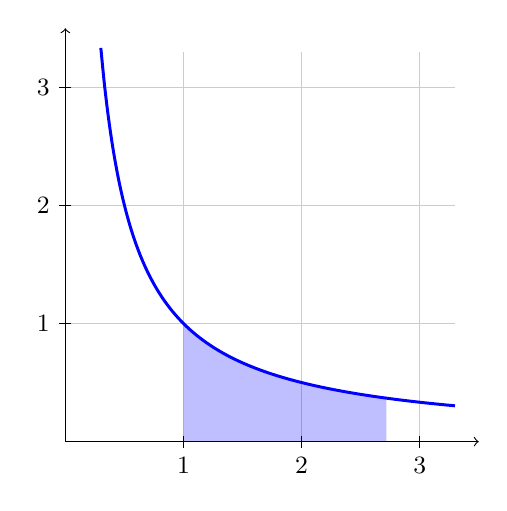
\begin{tikzpicture}[scale = 1.5]
    \draw [black!20, very thin] (0,0) grid (3.3,3.3);
    \fill [domain=1:e,
    smooth,
    blue,
    opacity = .25,
    samples = 100]
    (1,0) -- plot (\x, {pow(\x, -1)}) -- (e,0) -- cycle;
    \draw [domain=.3:3.3,
    smooth,
    line width = .25ex,
    blue,
    samples = 100]
    plot (\x, {pow(\x, -1)});
    \draw [->, thin] (0,0) -- (0,3.5);
    \draw [->, thin] (0,0) -- (3.5,0);
    \foreach \x in {1,2,3} {
      \draw (\x, .05) -- (\x, -.05) node [below]
      {\begin{small}$\x$\end{small}};
      \draw (.05, \x) -- (-.05, \x) node [left]
      {\begin{small}$\x$\end{small}};
    }
  \end{tikzpicture}
\end{center}

\begin{center}
  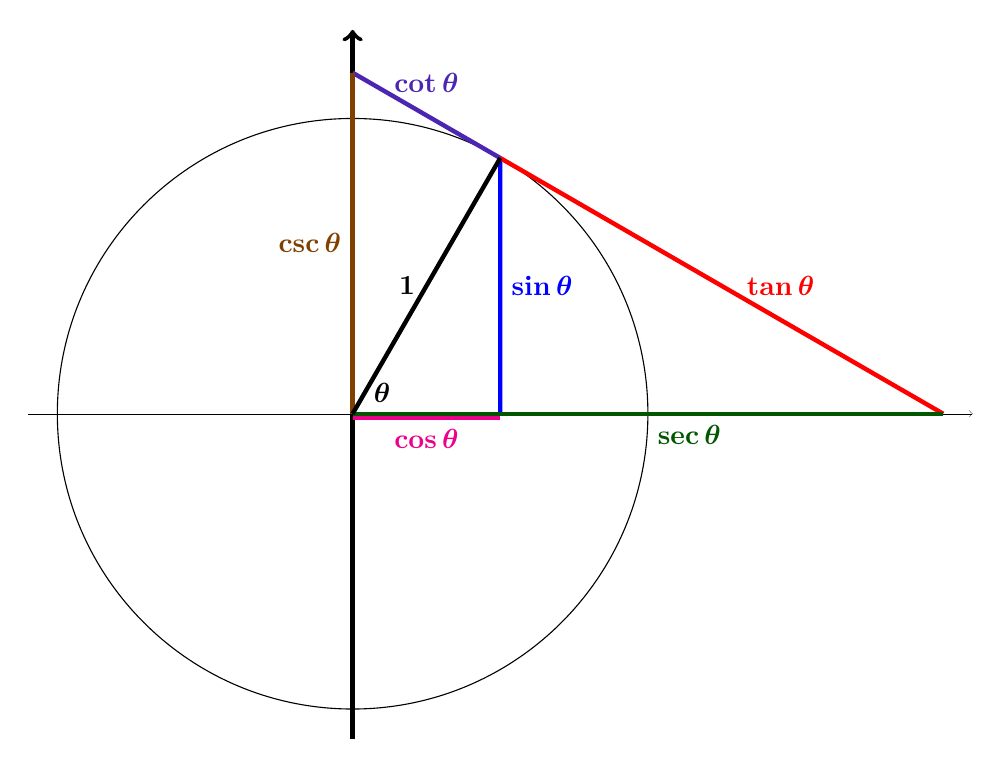
\begin{tikzpicture}[scale = 3.75]
    \draw [->, ultra thin] (-1.1,0) -- (2.1,0);
    \draw [->, ultra thick] (0,-1.1) -- (0,1.3);
    \draw (0,0) circle (1);
    \coordinate (A) at (0.5,0.86602540378);
    \boldmath
    \node at (.1,.07) {$\theta$};
    \draw [ultra thick, blue] (.5,0) to
    node [right] {$\sin \theta$} (A);
    \draw [ultra thick, red] (A) to
    node [right = 5] {$\tan \theta$} (2,0);
    \draw [ultra thick, black!66!green] (0,0) to
    node [below, xshift = 15] {$\sec \theta$} (2,0);
    \draw [ultra thick, magenta] (0,-.015) to
    node [below] {$\cos \theta$} (.5,-.015);
    \draw [ultra thick, orange!30!blue] (A) to
    node [above = 4] {$\cot \theta$} (0,1.155);
    \draw [ultra thick, black!50!orange] (0,0) to
    node [left] {$\csc \theta$} (0,1.155);
    \draw [ultra thick] (0,0) to node [left] {$1$} (A);
    \unboldmath
  \end{tikzpicture}
\end{center}

To access three dimensional coordinates, the \verb~tikz-3dplot~
package must be loaded in the preamble.

\begin{center}
  \tdplotsetmaincoords{25}{100}
  \begin{tikzpicture}[baseline,line join=bevel,scale = .5,tdplot_main_coords,
    hexface_style/.style={fill opacity=.8, fill=white, thick},
    pentface_style/.style={fill opacity=.4, fill=blue!50!black, thick}]

    \coordinate (A1) at (0,1,4.8541);
    \coordinate (A2) at (0,1,-4.8541);
    \coordinate (A3) at (0,-1,4.8541);
    \coordinate (A4) at (0,-1,-4.8541);

    \coordinate (B1) at (1,4.8541,0);
    \coordinate (B2) at (1,-4.8541,0);
    \coordinate (B3) at (-1,4.8541,0);
    \coordinate (B4) at (-1,-4.8541,0);

    \coordinate (C1) at (4.8541,0,1);
    \coordinate (C2) at (4.8541,0,-1);
    \coordinate (C3) at (-4.8541,0,1);
    \coordinate (C4) at (-4.8541,0,-1);

    \coordinate (D1) at (2, 4.23607, 1.61803);
    \coordinate (D2) at (2, 4.23607, -1.61803);
    \coordinate (D3) at (2, -4.23607, 1.61803);
    \coordinate (D4) at (2, -4.23607, -1.61803);
    \coordinate (D5) at (-2, 4.23607, 1.61803);
    \coordinate (D6) at (-2, 4.23607, -1.61803);
    \coordinate (D7) at (-2,-4.23607, 1.61803);
    \coordinate (D8) at (-2,-4.23607, -1.61803);

    \coordinate (E1) at (4.23607, 1.61803, 2);
    \coordinate (E2) at (4.23607, 1.61803, -2);
    \coordinate (E3) at (4.23607, -1.61803, 2);
    \coordinate (E4) at (4.23607, -1.61803, -2);
    \coordinate (E5) at (-4.23607, 1.61803, 2);
    \coordinate (E6) at (-4.23607, 1.61803, -2);
    \coordinate (E7) at (-4.23607, -1.61803, 2);
    \coordinate (E8) at (-4.23607, -1.61803, -2);

    \coordinate (F1) at (1.61803, 2, 4.23607);
    \coordinate (F2) at (1.61803, 2, -4.23607);
    \coordinate (F3) at (1.61803, -2, 4.23607);
    \coordinate (F4) at (1.61803, -2, -4.23607);
    \coordinate (F5) at (-1.61803, 2, 4.23607);
    \coordinate (F6) at (-1.61803, 2, -4.23607);
    \coordinate (F7) at (-1.61803, -2, 4.23607);
    \coordinate (F8) at (-1.61803, -2, -4.23607);

    \coordinate (G1) at (1, 3.61803, 3.23607);
    \coordinate (G2) at (1, 3.61803, -3.23607);
    \coordinate (G3) at (1, -3.61803, 3.23607);
    \coordinate (G4) at (1, -3.61803, -3.23607);
    \coordinate (G5) at (-1, 3.61803, 3.23607);
    \coordinate (G6) at (-1, 3.61803, -3.23607);
    \coordinate (G7) at (-1, -3.61803, 3.23607);
    \coordinate (G8) at (-1, -3.61803, -3.23607);

    \coordinate (H1) at (3.61803, 3.23607,1);
    \coordinate (H2) at (3.61803, 3.23607,-1);
    \coordinate (H3) at (3.61803, -3.23607,1);
    \coordinate (H4) at (3.61803, -3.23607,-1);
    \coordinate (H5) at (-3.61803, 3.23607,1);
    \coordinate (H6) at (-3.61803, 3.23607,-1);
    \coordinate (H7) at (-3.61803, -3.23607,1);
    \coordinate (H8) at (-3.61803, -3.23607,-1);

    \coordinate (I1) at (3.23607, 1, 3.61803);
    \coordinate (I2) at (3.23607, 1, -3.61803);
    \coordinate (I3) at (3.23607, -1, 3.61803);
    \coordinate (I4) at (3.23607, -1, -3.61803);
    \coordinate (I5) at (-3.23607, 1, 3.61803);
    \coordinate (I6) at (-3.23607, 1, -3.61803);
    \coordinate (I7) at (-3.23607, -1, 3.61803);
    \coordinate (I8) at (-3.23607, -1, -3.61803);

    \draw (H5) -- (E5) -- (C3) -- (C4) -- (E6) -- (H6) -- cycle;
    \draw (D6) -- (H6) -- (E6) -- (I6) -- (F6) -- (G6) -- cycle;
    \draw (G6) -- (D6) -- (B3) -- (B1) -- (D2) -- (G2) -- cycle;
    \draw (D2) -- (G2) -- (F2) -- (I2) -- (E2) -- (H2) -- cycle;
    \draw (A4) -- (F4) -- (I4) -- (I2) -- (F2) -- (A2) -- cycle;
    \draw (E4) -- (I4) -- (F4) -- (G4) -- (D4) -- (H4) -- cycle;
    \draw (D4) -- (G4) -- (G8) -- (D8) -- (B4) -- (B2) -- cycle;
    \draw (F8) -- (A4) -- (A2) -- (F6) -- (I6) -- (I8) -- cycle;
    \draw (H7) -- (E7) -- (C3) -- (C4) -- (E8) -- (H8) -- cycle;
    \draw (D8) -- (H8) -- (E8) -- (I8) -- (F8) -- (G8) -- cycle;
    \draw [pentface_style] (G2) -- (G6) -- (F6) -- (A2) -- (F2) -- cycle;
    \draw [pentface_style] (E4) -- (C2) -- (E2) -- (I2) -- (I4) -- cycle;
    \draw [pentface_style] (H5) -- (D5) -- (B3) -- (D6) -- (H6) -- cycle;
    \draw [pentface_style] (F4) -- (G4) -- (G8) -- (F8) -- (A4) -- cycle;
    \draw [pentface_style] (B4) -- (D7) -- (H7) -- (H8) -- (D8) -- cycle;
    \draw [pentface_style] (E8) -- (C4) -- (E6) -- (I6) -- (I8) -- cycle;

    \draw [hexface_style] (A1) -- (F5) -- (I5) -- (I7) -- (F7) -- (A3) -- cycle;
    \draw [hexface_style] (A1) -- (F1) -- (I1) -- (I3) -- (F3) -- (A3) -- cycle;
    \draw [hexface_style] (F1) -- (G1) -- (D1) -- (H1) -- (E1) -- (I1) -- cycle;
    \draw [hexface_style] (G1) -- (D1) -- (B1) -- (B3) -- (D5) -- (G5) -- cycle;
    \draw [hexface_style] (G5) -- (D5) -- (H5) -- (E5) -- (I5) -- (F5) -- cycle;
    \draw [hexface_style] (E1) -- (H1) -- (H2) -- (E2) -- (C2) -- (C1) -- cycle;
    \draw [hexface_style] (E3) -- (C1) -- (C2) -- (E4) -- (H4) -- (H3) -- cycle;
    \draw [hexface_style] (H3) -- (E3) -- (I3) -- (F3) -- (G3) -- (D3) -- cycle;
    \draw [hexface_style] (G7) -- (F7) -- (I7) -- (E7) -- (H7) -- (D7) -- cycle;
    \draw [hexface_style] (D3) -- (G3) -- (G7) -- (D7) -- (B4) -- (B2) -- cycle;
    \draw [pentface_style] (H4) -- (H3) -- (D3) -- (B2) -- (D4) -- cycle;
    \draw [pentface_style] (H1) -- (H2) -- (D2) -- (B1) -- (D1) -- cycle;
    \draw [pentface_style] (I7) -- (E7) -- (C3) -- (E5) -- (I5) -- cycle;
    \draw [pentface_style] (G3) -- (F3) -- (A3) -- (F7) -- (G7) -- cycle;
    \draw [pentface_style] (A1) -- (F1) -- (G1) -- (G5) -- (F5) -- cycle;
    \draw [pentface_style] (E1) -- (I1) -- (I3) -- (E3) -- (C1) -- cycle;
  \end{tikzpicture}
\end{center}

\end{document}
